\section{Theoretical Overview}
Path planning in modern video games often involves exploring highly regular 
environments such as cities, sewers or dungeons.
These locales tend to be topographically simple and are frequently comprised only
of empty connected rooms.
It may be somewhat surprising therefore to discover that the canonical A* 
algorithm\cite{hart68} has great difficulties in such domains .
The main problem encountered by A* when traversing across an empty or near-empty 
room is that all generated nodes will have very similar or even identical f-costs
(we gave an example of this behaviour in Figure \ref{fig-emptymap}(a)).
To preserve optimality A* must expand all such nodes until it can prove they do 
not appear on the optimal path.
%Figure \ref{fig-oha_contrast}(a) illustrates such a case; 
%notice that A* explores almost half the map. 
\begin{figure*}[htbp]
	\label{fig-oha_contrast}
	\vspace{-4pt}
       \begin{center}
           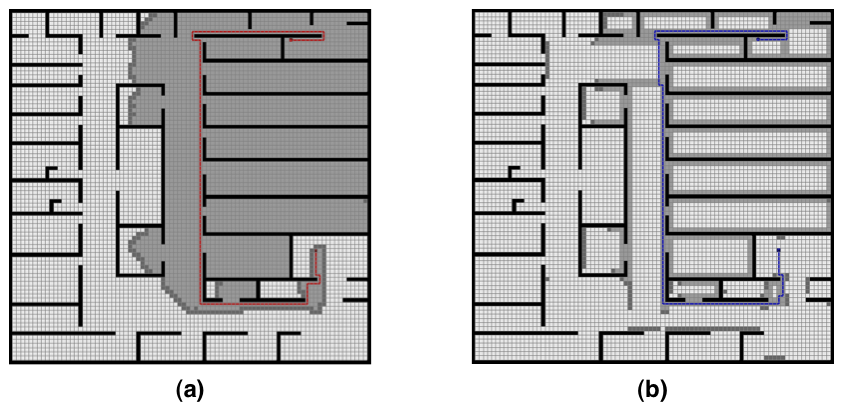
\includegraphics[scale=0.60, trim = 10mm 10mm 10mm 0mm]{diagrams/oha_contrast.png}
       \end{center}
	\vspace{-3pt}
       \caption{\textbf{(a)} A* solving a problem on a typical ($86\times88$) game map. 
Expanded nodes are marked light grey while nodes at the frontier of the search are dark grey.
\textbf{(b)} OHA* solving the same problem. A number of large clusters have been identified (not
all shown) and the algorithm only considers nodes along their perimeter.}
       \label{fig-ohacontrast}
	\vspace{-15pt}
\end{figure*}

\par
To overcome these difficulties we propose the following simple strategy:
instead of exploring the interior of an empty room expand only nodes along the
perimeter. We claim that this approach preserves optimality when searching in 
4-connected grid maps. 
Consider the following argument:

\begin{mylemma}
\label{thm-roomtraversal}
Every optimal path running through the interior of an empty 4-connected rectangular 
room $R$ is dominated by another 
optimal path involving only nodes on the perimeter of $R$.
\end{mylemma}
\begin{proof}
Let $s$ and $g$ correspond to a start and goal location such that $s, g \in R$.
There are two possible reasons for expanding nodes in $R$: 
$g$ is the final goal state and thus contained in the interior of $R$ or,
$g$ is an intermediate node on optimal path which passes through $R$.
We will show that in both cases there is no need to expand any nodes from the interior of $R$.
\par
First, suppose $g$ is the final goal and found in the interior of $R$ 
(as per Figure \ref{fig-roomtraversal}(a)).
In this case we can simply use a manhattan heuristic to exactly calculate $h^*(s, g)$.
Since $R$ is empty the heuristic is perfectly informed and we may generate $g$
as a direct \emph{macro successor} of $s$ without expanding any nodes from the interior of $R$.
\par
Next, suppose $s$ is located in the interior of $R$ (as per Figure \ref{fig-roomtraversal}(b)).
Further, suppose that $g$ is an intermediate node on a path through $R$ and thus
located on the perimeter of $R$.
We proceed by expanding $s$ to generate the macro successor set 
$\Gamma(s) = \lbrace s_{1}', s_{2}', s_{3}', s_{4}'\rbrace$ where each $s_{i}'$ is 
is the closest perimeter node to $s$ along each of the four sides of $R$.
Since $h^*$ is perfectly informed the cost of each macro edge 
$c(s, s_{i}') = h^*(s, s_{i}')$ is optimal.
Further, since $g$ is on the perimeter of $R$, there must exist a path $\pi(s_{i}', g)$ 
such that the cost of $\pi(s, g) = \pi(s, s_{i}') + \pi(s_{i}', g)$ is optimal.
\par
Finally, suppose that $s$ and $g$ are both located on the perimeter of $R$ 
(as in Figure \ref{fig-roomtraversal}(c)) and that $g$ is again an intermediate node.
If $g$ is on the same side of the perimeter to $s$ or on one of the two orthogonal sides 
it follows that we can find an optimal length path between them by the successive expansion of 
nodes adjacent to $s$ along the perimeter.
Suppose however that $g$ is somewhere on the opposide side of $R$.
In this case we can generate a single macro successor $s'$ which appears on the 
perimeter of $R$ directly opposite to $s$.
It now becomes trivial to show that there exists a path $\pi(s',g)$ and, 
since since $h^*$ is perfectly informed, that the cost of  
$\pi(s, g) = \pi(s, s') + \pi(s', g)$ is optimal.
\end{proof}

\begin{figure}[htbp]
	\label{fig-roomtraversal}
	\vspace{-4pt}
       \begin{center}
           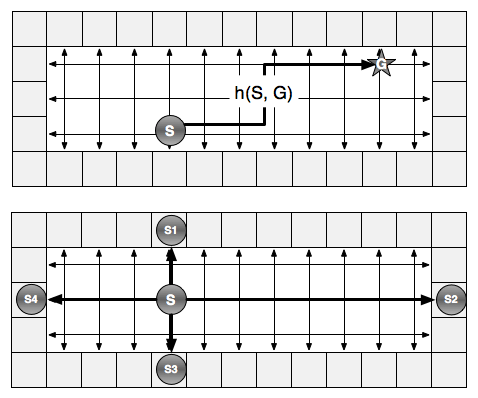
\includegraphics[scale=0.34, trim = 10mm 10mm 10mm 0mm]{diagrams/roomtraversal.png}
       \end{center}
	\vspace{-3pt}
       \caption{The three cases which must be considered in order to prove that 
			optimal traversal of an empty room is possible using only nodes from the perimeter.
			Dashed lines represent macro successors and solid lines represent segments of optimal
			paths that are eventually found}
       \label{fig-ohacontrast}
	\vspace{-15pt}
\end{figure}

A direct corrolary Lemma \ref{thm-roomtraversal} is that we can prune from consideration
all nodes from the interior of $R$ and limit ourselves to those nodes appearing along its perimeter.
In light of this result we propose the following hierarchical search strategy for finding shortest 
paths in 4-connected grid maps:

\begin{enumerate}
\item{\label{oha-step1} Preprocess a 4-connected grid map in order to construct a set of adjacent empty rooms such that 
each room is rectangular in shape and each tile on the map is assigned to exactly one room. }
\item{\label{oha-step2} Begin the search by expanding the start node as described in 
Lemma \ref{thm-roomtraversal} in order to generate the set 
$\Gamma(s) = \lbrace s_{1}', s_{2}', s_{3}', s_{4}'\rbrace$ which are added to the open list. }
\item{\label{oha-step3} Using any graph search algorithm evaluate the set of open nodes.}
\item{\label{oha-step4} When expanding a node $x$ that is not in the goal cluster generate the set 
$\Gamma(x) = \lbrace p, q, x' \rbrace$ as described in Lemma \ref{thm-roomtraversal} and updating the open
list as required.} 
\item{\label{oha-step5} When expanding a node $s$ that is in the goal cluster generate $g$ directly as 
described in Lemma \ref{thm-roomtraversal}} 
\item{Repeat steps \ref{oha-step3}-\ref{oha-step5} until either the goal is found (in which case return
the path) or all nodes have been evaluated (in which case return failure).}
\end{enumerate}
When the graph search algorithm at step \ref{oha-step3} is A* we term the resulting algorithm 
Optimal Hierarchical A* (or simply OHA*).


\begin{mytheorem}
OHA* is optimal. 
\end{mytheorem}
\begin{proof}
To prove this claim we have to show that for every optimal length path $\pi(s, g)$ 
on a 4-connected grid map, which starts at node $s$ and terminates at node $g$, 
there exists an equivalent path using only nodes from the perimeter of empty rooms.
The proof is almost immediate following Lemma \ref{thm-roomtraversal}. 
We will show it is true using a constructive approach.
\par
Every optimal length path $\pi(s, g)$  involves some set of traversable nodes.
However, every traversable node also appears in an empty room.
Thus, we have to to show that for every segment of an optimal path which passes through 
an empty room there is an identical segment of equal length, starting and ending
with the same pair of nodes, but which never visits the interior of any room.
This is exactly the problem we discussed in Lemma \ref{thm-roomtraversal} 
so we know that such a segment exists for any pair of tiles on the perimeter of any room.
Therefore it must be that for every optimal length path in a 4-connected grid map there must exist
another optimal length path, starting and ending with the same pair of nodes, which
only visits nodes on the perimeter of empty rooms. 
\end{proof}

To highlight how well OHA* can work in practice consider the example game map in Figure 
\ref{fig-oha_contrast}. 
The topograpy of this map is typical of what one might expect in a modern roleplaying game
\footnote{Infact, most video game maps tend to be somewhat bigger than our example but for demonstration 
purposes it is quite sufficient.};
there are many rooms and corridors and many entrances to connect them.
In Figure \ref{fig-oha_contrast}(a) we show A* solving what appears to be quite a simple problem. 
Unfortunately obtaining the optimal solution required expanding over half the nodes on the map.
Figure \ref{fig-oha_contrast}(b) shows the same problem being solved by OHA*.
We were able to prune away large sections of the map by taking advantage of the fact that
such nodes never need to be expanded in order to retain optimality.
In this case OHA* expands less than $\frac{1}{3}$ of the area explored by A* and returns
a solution 4 times faster.

